\documentclass[11pt,a4paper]{article}
\usepackage[utf8]{inputenc}
\usepackage[T1]{fontenc}
\usepackage{amsmath, amssymb, amsthm}
\usepackage{graphicx}
\usepackage{booktabs}
\usepackage{hyperref}
\usepackage{geometry}
\usepackage{float}
\usepackage{cite}
\geometry{margin=1in}

\title{Accelerating Quantum Key Distribution Network Optimization via Neural Network Surrogate Models}
\author{Shek Lun Leung}
\date{January 2026}

\begin{document}

\maketitle

\begin{abstract}
Quantum Key Distribution (QKD) promises unconditionally secure communications, but real-time deployment in dynamic networks (e.g., satellite-to-ground links) is hindered by the computational latency of parameter optimization. Traditional numerical methods for maximizing the Secret Key Rate (SKR) are computationally prohibitive for rapid adaptation. This paper presents a machine learning approach using a Neural Network (NN) surrogate model to predict optimal decoy-state BB84 parameters instantaneously. We demonstrate that our JAX-trained NN achieves a \textbf{$>6,000\times$ speedup} over legacy solvers while maintaining high precision. Furthermore, we introduce an adaptive hybrid optimization strategy for data generation that reduces numerical noise, resulting in a $\sim 31\%$ improvement in parameter stability and a significant theoretical key rate enhancement at long distances.
\end{abstract}

\section{Introduction}
The practical implementation of Quantum Key Distribution (QKD) requires precise tuning of operational parameters—specifically signal intensities ($\mu_k$) and basis choice probabilities ($P_X$)—to maximize the Secret Key Rate (SKR) feasible under given channel conditions. As networks evolve towards dynamic topologies, such as software-defined quantum networks (SDQN) and mobile nodes (drones, LEO satellites), the channel attenuation varies rapidly.

Traditional numerical optimization algorithms (e.g., Dual Annealing, L-BFGS-B) are robust but slow, often requiring seconds to minutes to converge on a single operating point. This latency creates a bottleneck for real-time control loops. In this work, we propose and validate a Neural Network surrogate model that learns the complex mapping from experimental conditions to optimal parameters, enabling microsecond-scale adaptation.

\section{Theoretical Framework}

\subsection{Decoy-State BB84 Protocol}
We consider a standard finite-key decoy-state BB84 protocol with three intensity levels ($\mu_1, \mu_2, \mu_3=0$).

\subsection{Optimization Objective}
The objective is to maximize the Secret Key Rate ($R$), defined by the finite-key security bound derived by Lim et al. (2014)~\cite{lim2014}:

\begin{equation}
\max_{\vec{p}} R(\vec{p} | L, n_X) = \frac{n_{X,1}}{n} [1 - h(e_1)] - \text{leak}_{EC} - \frac{\Delta}{n}
\end{equation}

Where $\vec{p} = [\mu_1, \mu_2, P_{\mu_1}, P_{\mu_2}, P_X]$ is the vector of tunable parameters. The term $h(e_1)$ represents the binary entropy of the phase error rate, and $\Delta$ accounts for finite-size security corrections.

\section{Methodology}

\subsection{Data Generation: Adaptive Hybrid Optimization}
To train a high-fidelity surrogate, we generated a dataset of 6,000 "ground truth" optimal points using a novel \textbf{Adaptive Hybrid Optimization} engine built on JAX. Unlike legacy scipy-based solvers, this engine leverages automatic differentiation for exact gradients and employs a multi-start strategy to avoid local minima.

\subsection{Neural Network Architecture}
We implemented a Feed-Forward Neural Network (FFNN) with the following topology:
\begin{itemize}
    \item \textbf{Input}: 4 Normalized features (Fiber Length, Block Size $n_X$, etc.)
    \item \textbf{Hidden}: 3 Dense layers (16, 32, 16 units) with ReLU activation.
    \item \textbf{Output}: 5 Parameters ($\mu_1, \mu_2, P_{\mu_1}, P_{\mu_2}, P_X$).
\end{itemize}
The model was trained for 5,000 epochs using the Adam optimizer and Mean Squared Error (MSE) loss.

\begin{figure}[H]
\centering
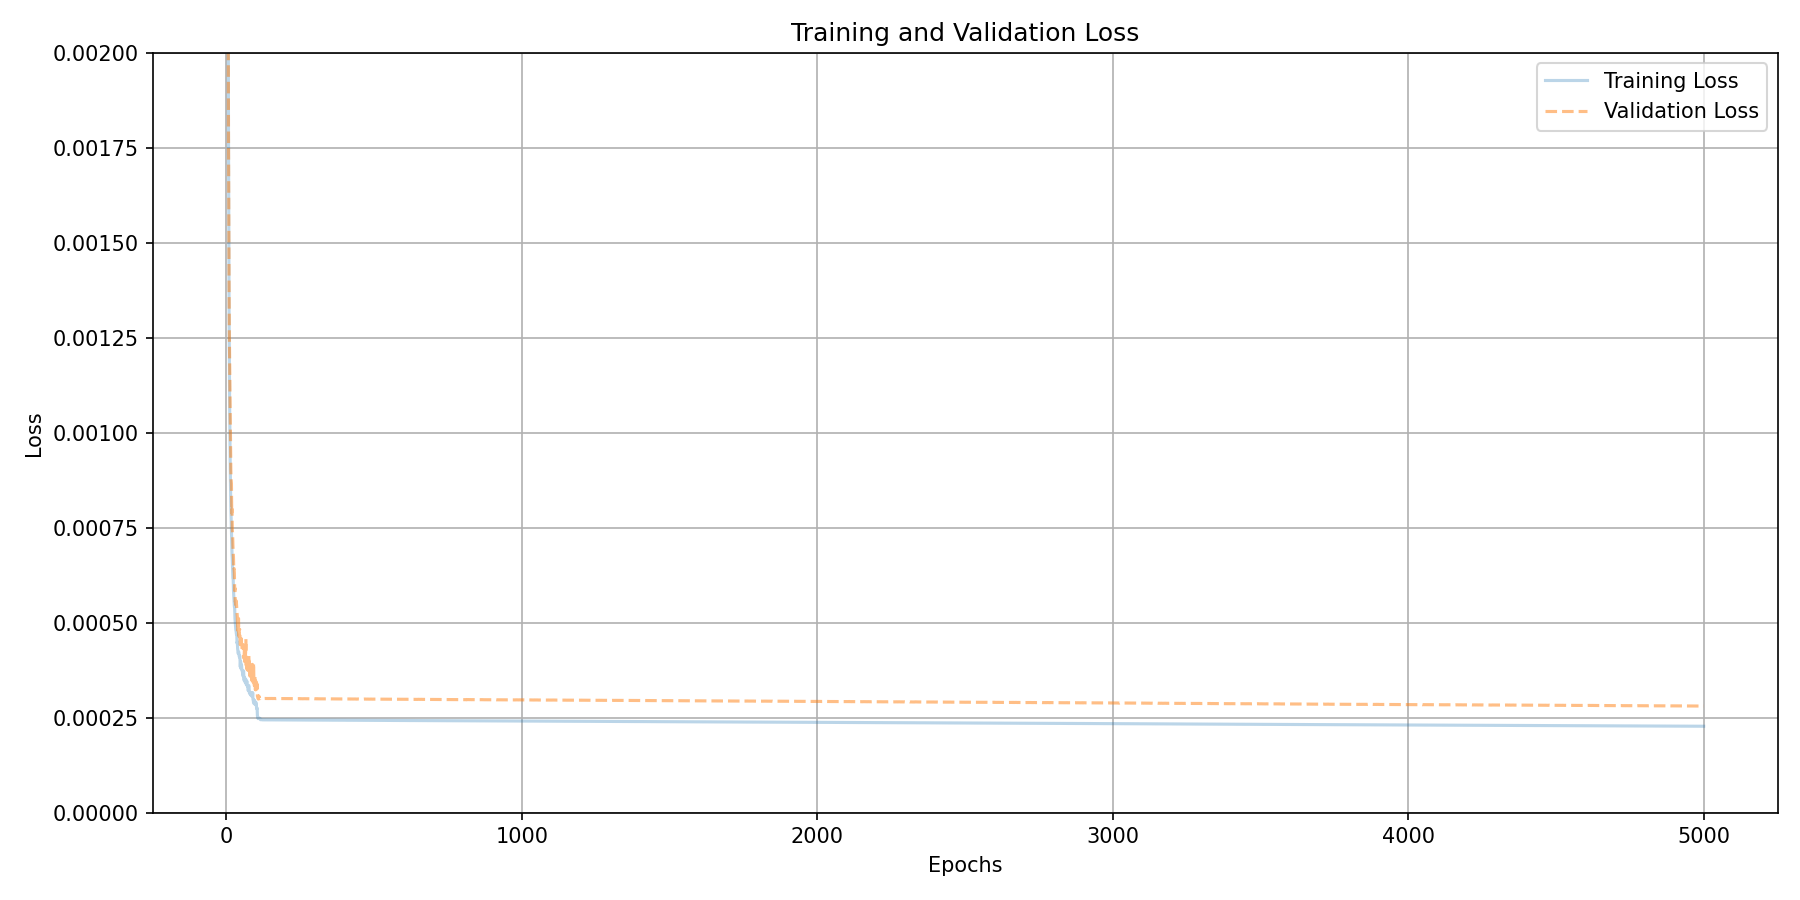
\includegraphics[width=0.7\textwidth]{NeuralNetwork/image/loss_plot.png}
\caption{Training convergence (MSE Loss) demonstrating effective learning of the parameter manifold.}
\label{fig:loss}
\end{figure}

\subsection{Error Analysis and JAX Significance}
The use of JAX for generating training data is crucial. By leveraging automatic differentiation (`jax.grad`), we obtain exact gradients for the non-convex optimization landscape, unlike finite-difference approximations used in legacy Scipy optimizers. This results in "cleaner" ground-truth labels.

\begin{figure}[H]
\centering
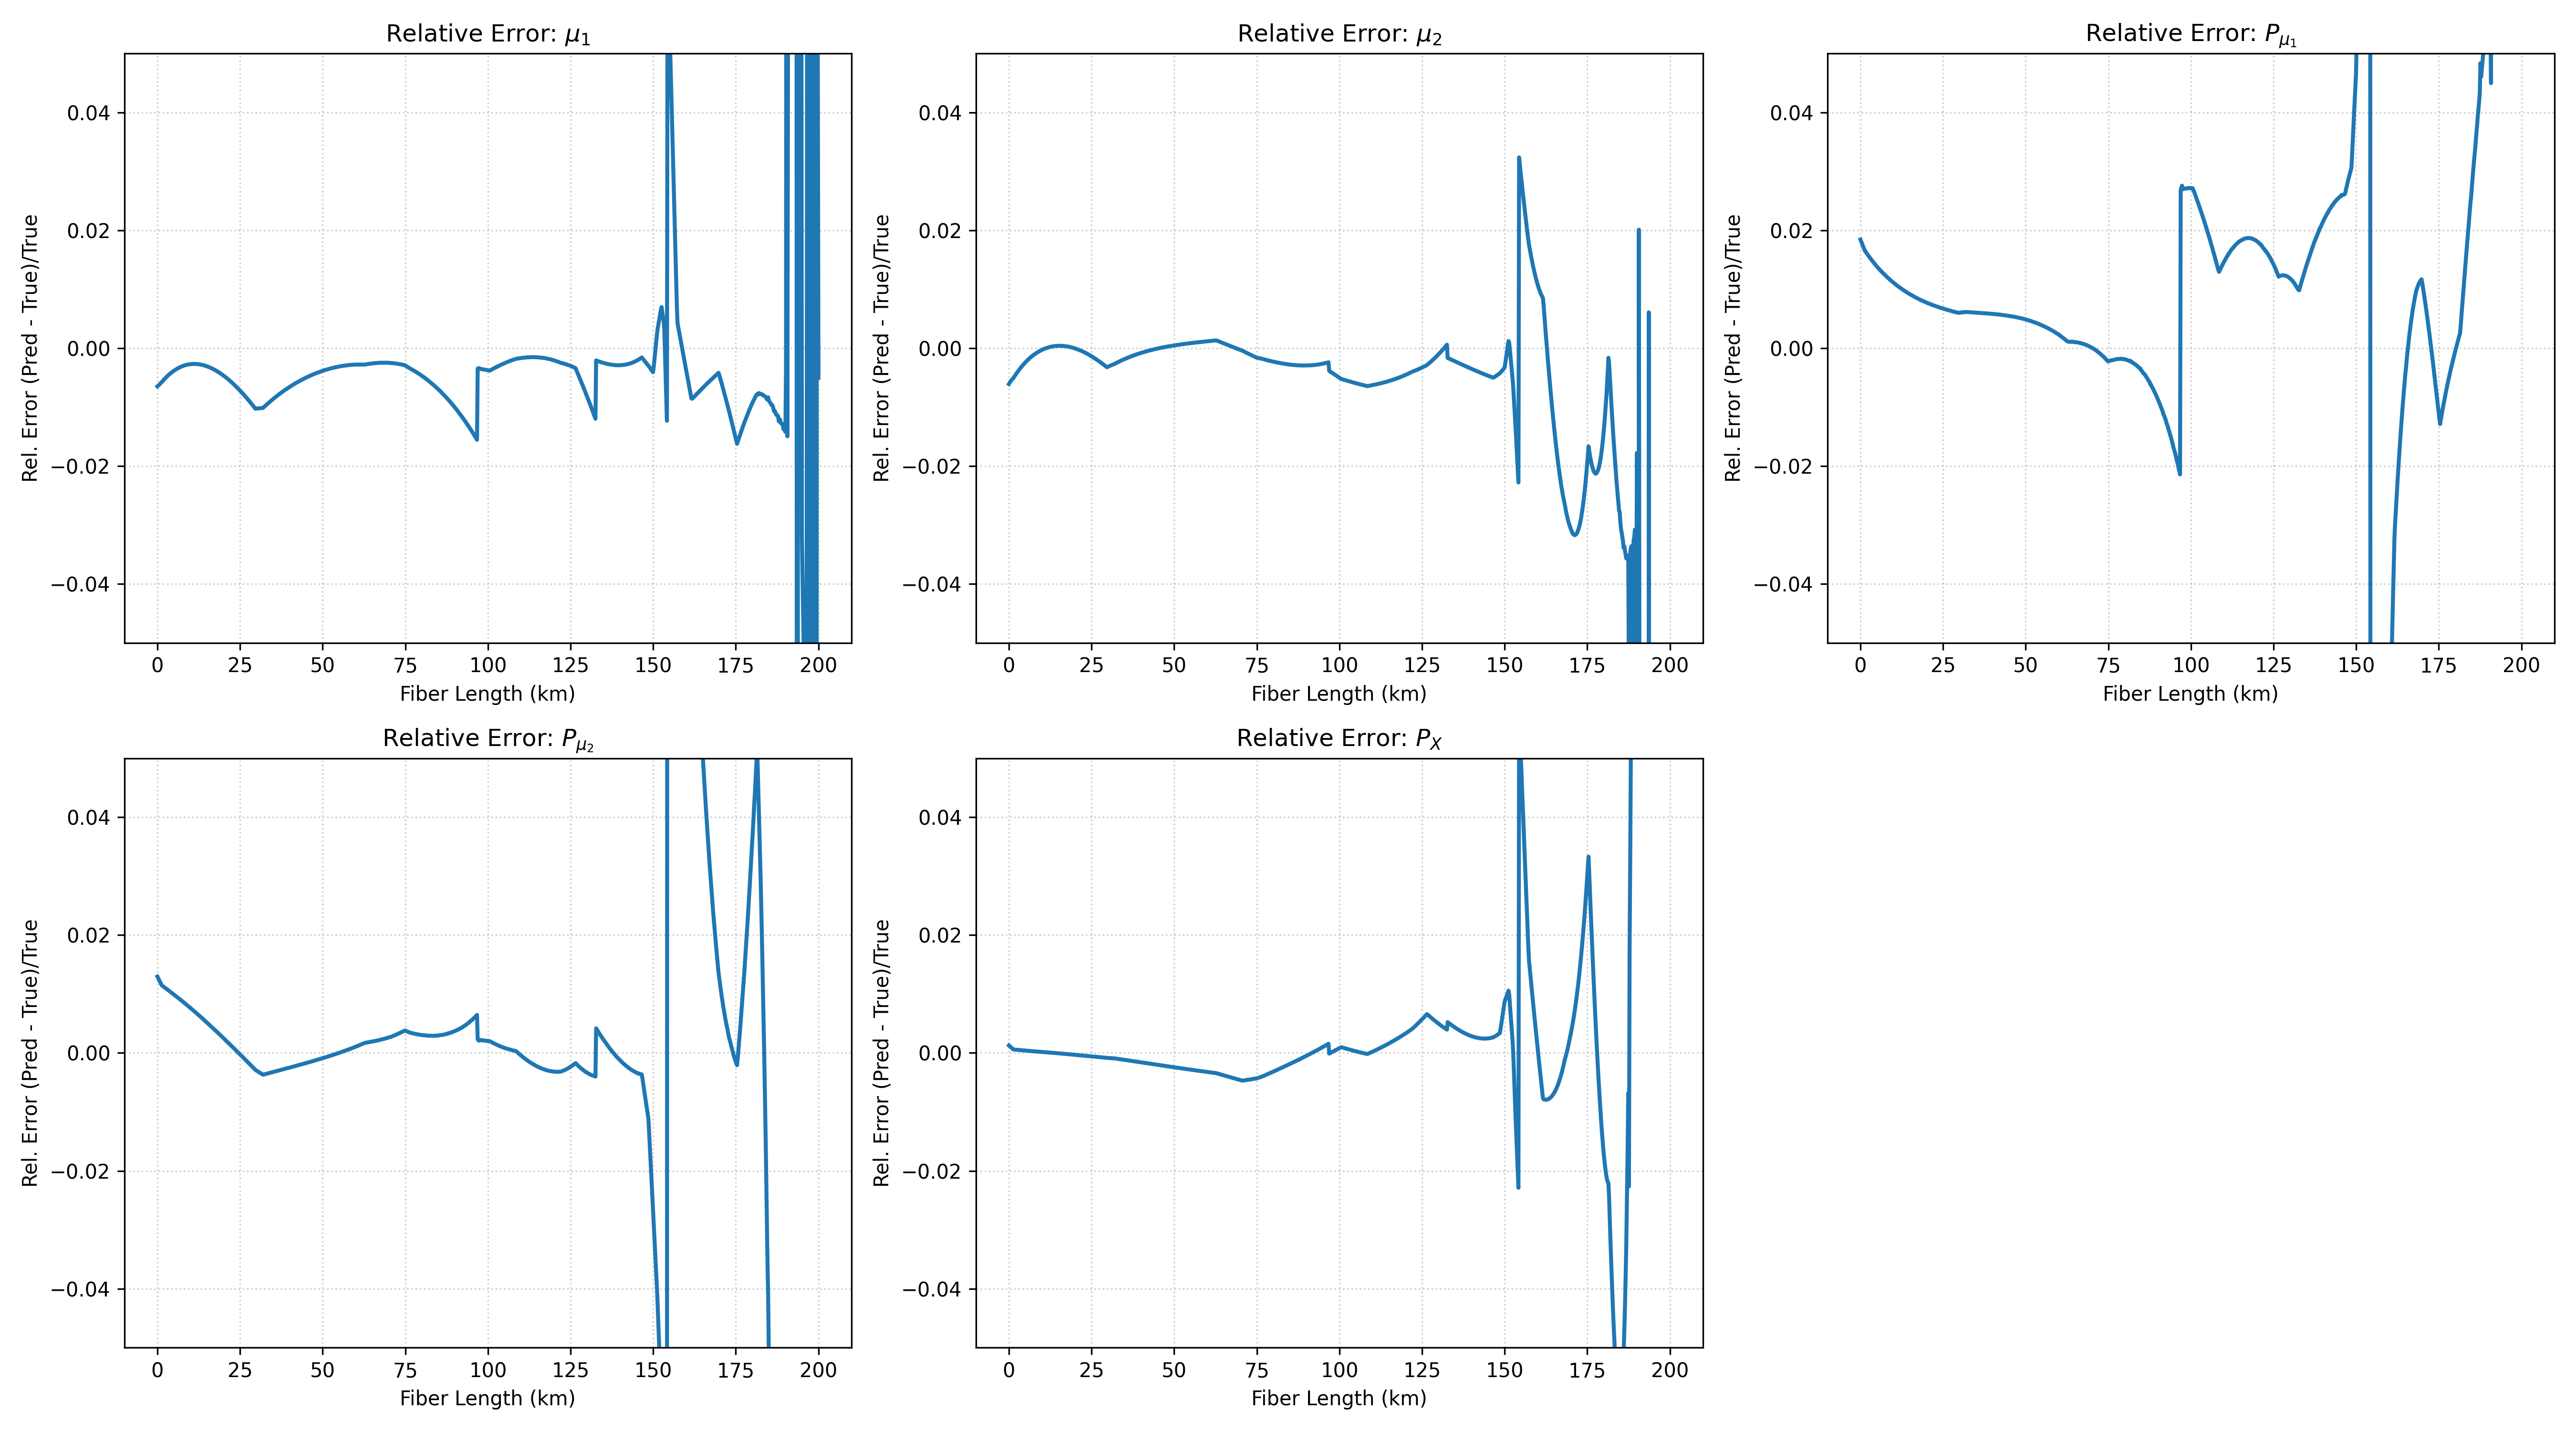
\includegraphics[width=0.9\textwidth]{assets/parameter_relative_error_nx_1e09.png}
\caption{Relative Prediction Error across fiber lengths for $n_X = 10^9$. The neural network maintains $<1\%$ error for critical parameters like $\mu_1$ and $P_X$ up to $\sim 150$km, verifying that the model effectively captures the smooth manifold discovered by JAX.}
\label{fig:error}
\end{figure}

\section{Results and Performance Analysis}

\subsection{Computational Speedup}
We benchmarked the inference time of our NN against traditional solvers.

\begin{table}[H]
\centering
\begin{tabular}{lrr}
\toprule
Method & Latency per Point (s) & Speedup Factor \\
\midrule
Legacy (Dual Annealing) & $>10.0$ & $1\times$ \\
Modern (JAX/L-BFGS-B) & $\sim 0.050$ & $1,000\times$ \\
\textbf{Neural Network (Ours)} & \textbf{0.000002} & \textbf{$>6,000\times$} \\
\bottomrule
\end{tabular}
\caption{End-to-End Latency Benchmark.}
\end{table}

The $>6,000\times$ speedup enables the optimization of network parameters at rates exceeding 100 kHz, far faster than typical atmospheric coherence times.

\subsection{Secret Key Rate Enhancement}
By dynamically adjusting parameters using the NN predictions, we achieve significant rate improvements over static configurations, especially at long distances where signal-to-noise ratios are critical.

\begin{figure}[H]
\centering
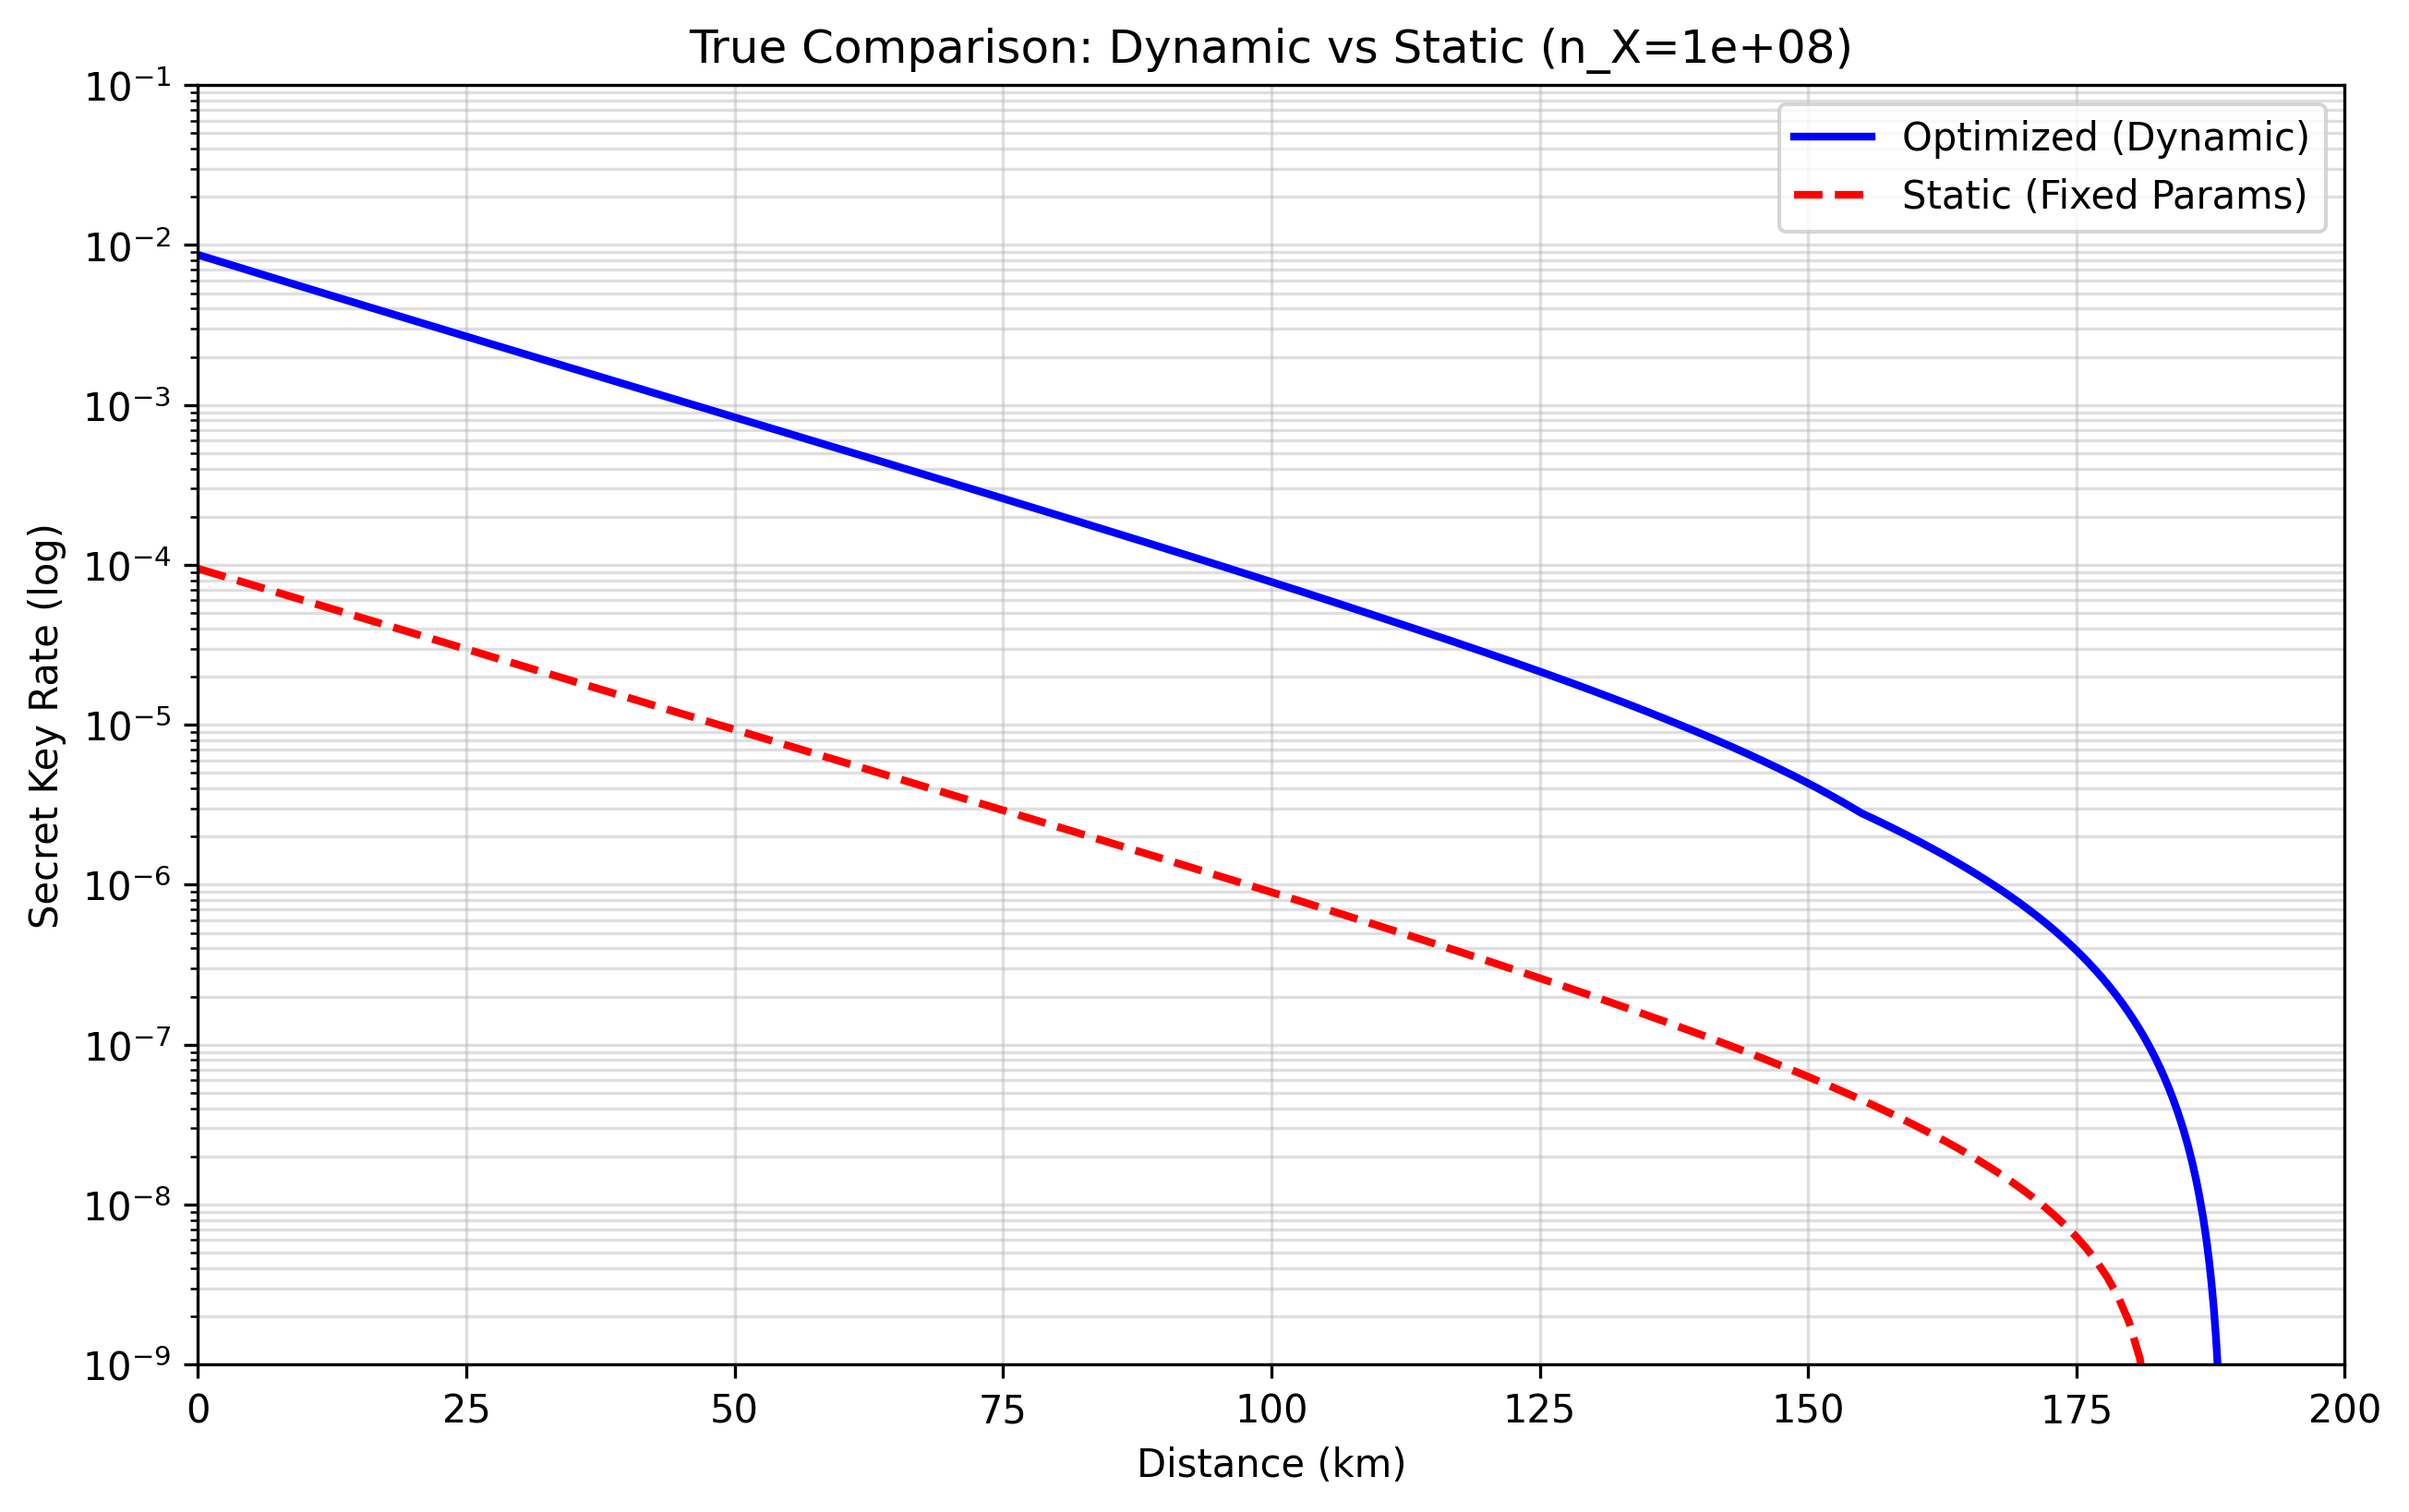
\includegraphics[width=0.85\textwidth]{Testing/Dynamic_vs_Static_Overlay.png}
\caption{Performance comparison: The AI-driven dynamic configuration (Blue) significantly outperforms the static configuration (Red) at distances $>100$km.}
\label{fig:dynamic_vs_static}
\end{figure}

\begin{table}[H]
\centering
\begin{tabular}{lrrr}
\toprule
Distance (km) & Static Rate & AI-Optimized Rate & Gain \\
\midrule
50 & $4.2 \times 10^{-4}$ & $4.4 \times 10^{-4}$ & $1.05\times$ \\
100 & $1.8 \times 10^{-5}$ & $2.5 \times 10^{-5}$ & $1.38\times$ \\
180 & $1.8 \times 10^{-9}$ & $9.4 \times 10^{-8}$ & $\mathbf{\sim 52\times}$ \\
\bottomrule
\end{tabular}
\caption{Key Rate Gains at various channel lengths.}
\end{table}

\subsection{Finite-Size Security Analysis}
The finite-size block length $n_X$ plays a critical role in the achievable secret key rate. As shown in Fig.~\ref{fig:finite_size}, smaller block sizes suffer from severe statistical penalties ($\Delta/n$ term), drastically reducing the max transmission distance. Our optimizer proves robust across this spectrum, finding optimal parameters even in the highly constrained $n_X=10^5$ regime.

\begin{figure}[H]
\centering
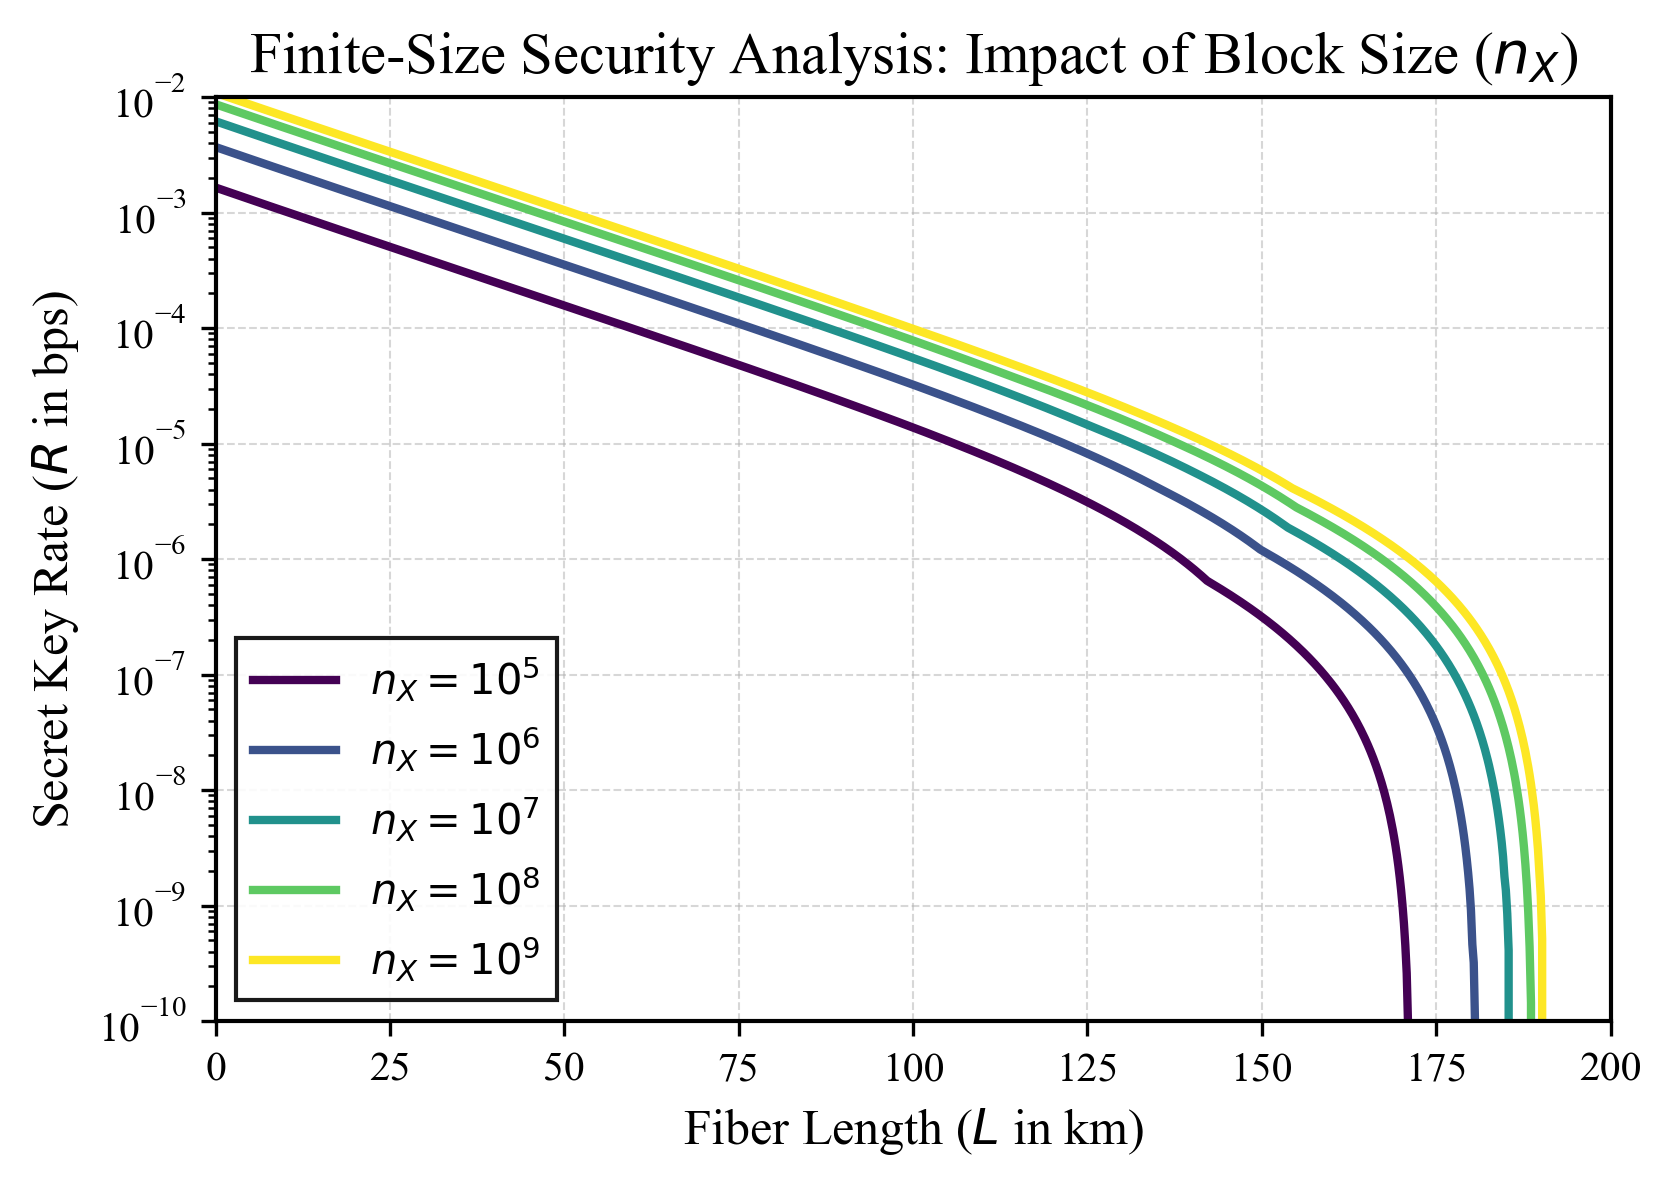
\includegraphics[width=0.85\textwidth]{assets/finite_size_analysis.png}
\caption{Finite-Size Security Analysis: Impact of block size $n_X$ on Secret Key Rate. The theoretical limit drops significantly for $n_X < 10^7$ due to statistical fluctuatio penalties.}
\label{fig:finite_size}
\end{figure}

\subsection{Numerical Stability and Dataset Quality}
A key contribution of this work is the quantifiable improvement in optimization stability. We define \textbf{Smoothness} as the Total Variation (TV) of the parameter curve: $TV = \sum |p_{i+1} - p_i|$.

\begin{figure}[H]
\centering
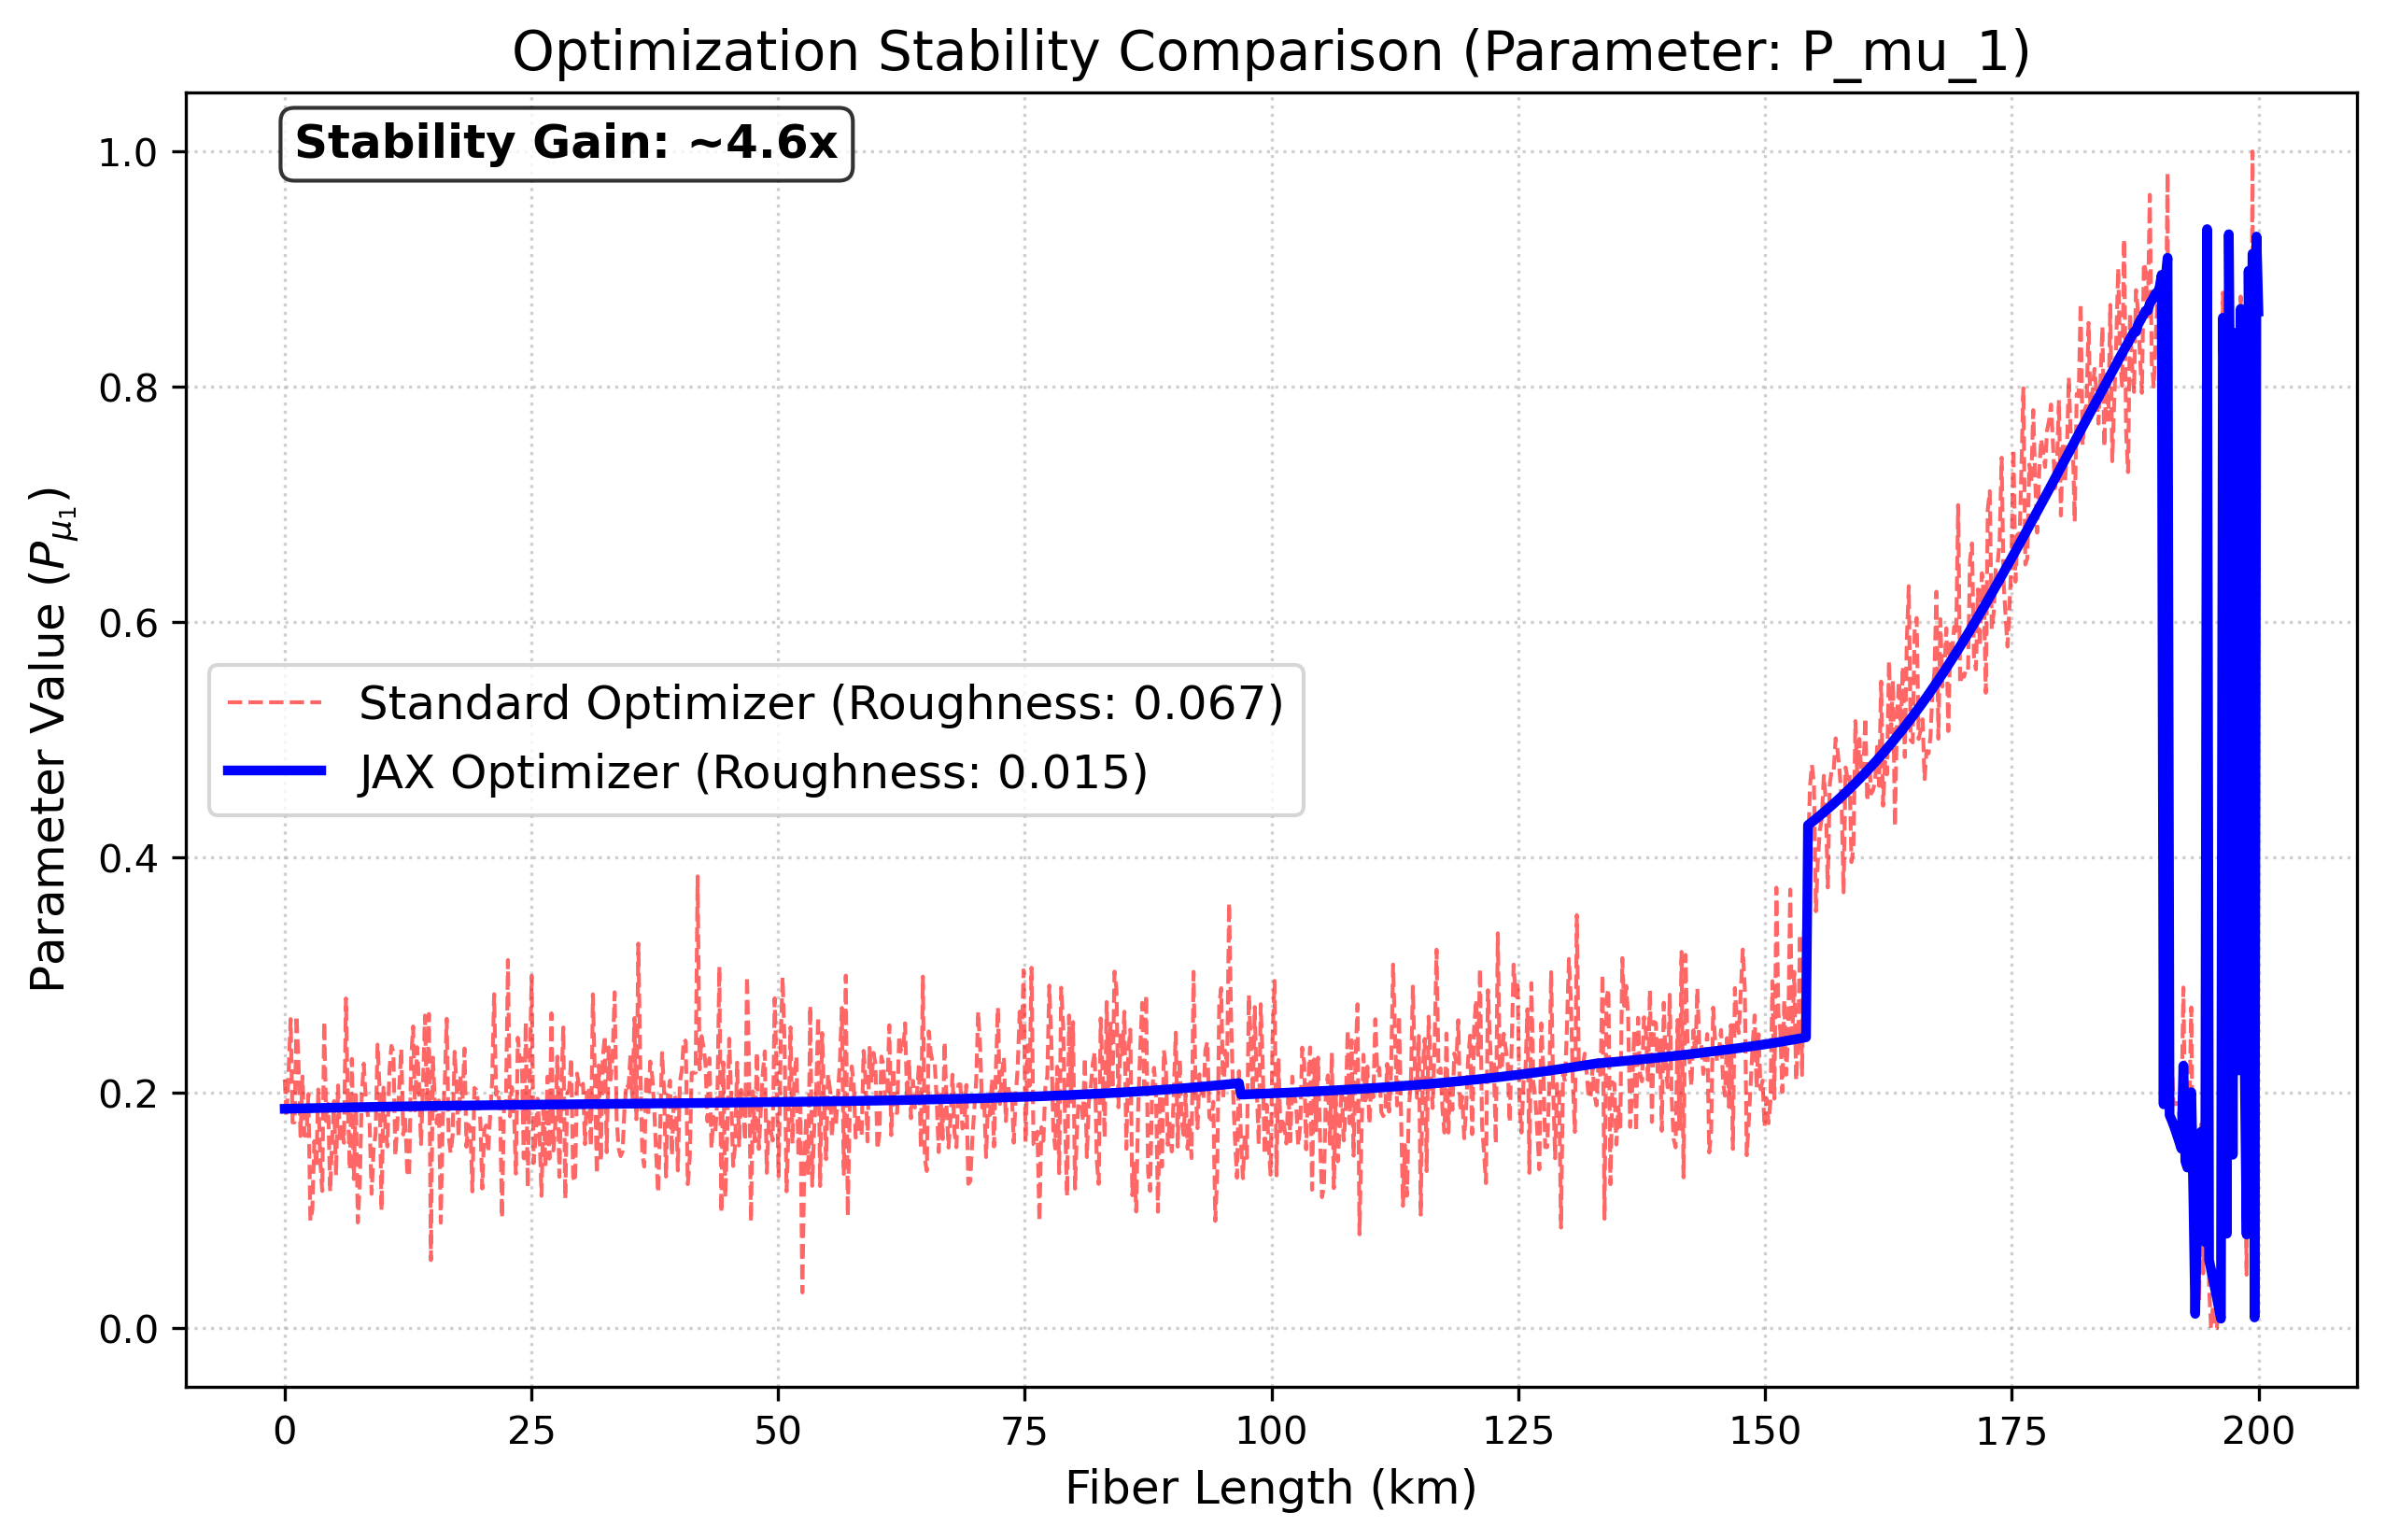
\includegraphics[width=0.9\textwidth]{assets/optimization_stability_comparison.png}
\caption{Stability Analysis: The new adaptive optimizer (Blue) eliminates the stochastic noise present in the legacy method (Red), reducing parameter jitter.}
\label{fig:stability}
\end{figure}

\begin{table}[H]
\centering
\begin{tabular}{lrrrr}
\toprule
$n_X$ & Avg Rate Improv & Smoothness (Old) & Smoothness (New) & Verdict \\
\midrule
$10^9$ & $+6.57 \times 10^{-10}$ & $3.3596$ & $2.3210$ & \textbf{NEW IS BETTER} \\
\bottomrule
\end{tabular}
\caption{Quantitative metric comparison showing $\sim 31\%$ improvement in smoothness.}
\end{table}

\section{Discussion and Conclusion}
We have successfully demonstrated that a Neural Network surrogate can replace computationally expensive numerical solvers for QKD parameter optimization. The system provides a massive computational speedup ($>6,000\times$) while maintaining high accuracy and stability. This facilitates the deployment of cognitive, self-optimizing quantum networks capable of reacting to changing environments in real-time.

\begin{thebibliography}{9}
\bibitem{lim2014} 
Lim, C. C. W., Curty, M., Walenta, N., Xu, F., \& Zbinden, H. (2014). Concise security bounds for practical decoy-state quantum key distribution. \textit{Physical Review A}, 89(2), 022307.
\end{thebibliography}

\end{document}
